%%%%%%%%%%%%%%%%%%%%%%%%%%%%%%%%%%%%%%%%%%
% Engineering problems / LaTeX Template
%		Semester 6
%		Institut d'Optique Graduate School
%%%%%%%%%%%%%%%%%%%%%%%%%%%%%%%%%%%%%%%%%%
%	6N-IntNum-BlocVI
%%%%%%%%%%%%%%%%%%%%%%%%%%%%%%%%%%%%%%%%%%
%
% Created by:
%	Julien VILLEMEJANE - 20/nov/2025
%	
%
%%%%%%%%%%%%%%%%%%%%%%%%%%%%%%%%%%%%%%%%%%
% Professional Newsletter Template
% LaTeX Template
% Version 1.0 (09/03/14)
%
% Created by:
% Bob Kerstetter (https://www.tug.org/texshowcase/) and extensively modified by:
% Vel (vel@latextemplates.com)
% 
% This template has been downloaded from:
% http://www.LaTeXTemplates.com
%
% License:
% CC BY-NC-SA 3.0 (http://creativecommons.org/licenses/by-nc-sa/3.0/)
%
%%%%%%%%%%%%%%%%%%%%%%%%%%%%%%%%%%%%%%%%%

\documentclass[a4paper,11pt,titlepage]{article} % The default font size is 10pt; 11pt and 12pt are alternatives

%%%%%%%%%%%%%%%%%%%%%%%%%%%%%%%%%%%%%%%%%%%%%%%%%%%%%%%%%%%%%%%%%%%%%%%%%%%%%%%%%%%%%%%%%%%%%%%%%%%%%%%%%%%%%%%%%%%%%%%%%%%%%%%%%%%%%%%%%%%%%%%%%%%%%%%%%%%%%%%%%%%%%%%%%%%%%%%%%%%%%%%%%%%%%%%%%%%%%%%%%%%%%%%%%%%%%%%%%%%%%%%%%%%%%%%%%%%%%%%%%%%%%%%%%%%%
\usepackage{../opto_elec_villemejane}

%%%%%%%%%%%%%%%%%%%%%%%%%%%%%%%%%%%%%%%%%%%%%%%%
%%%%%%%%%%%%%%%%%%%%%%%%%%%%%%%%%%%%%%%%%%%%%%%%
\begin{document}


% Page de garde
\begin{titlepage}

\begin{center}
	\begin{minipage}{2.5cm}
	\begin{center}
		
\includegraphics[width=8cm]{../images/Logo-LEnsE.png}
	\end{center}
\end{minipage}\hfill
\begin{minipage}{10cm}
	\begin{center}
	\textbf{Institut d'Optique Graduate School }\\[0.1cm]
    \textbf{\textsc{\Large Interfaçage Numérique}}


	\end{center}
\end{minipage}\hfill


\vspace{1cm}
{\large \bfseries Travaux Pratiques} \\[0.2cm]
Semestre 5

\vspace{1cm}
% Title
\rule{\linewidth}{0.3mm} \\[0.4cm]
{ \huge \bfseries\color{violet_iogs} Vision Industrielle \\[0.4cm] }
\rule{\linewidth}{0.3mm} \\[0.2cm]
{ \large \bfseries\color{violet_iogs} Ressources}
\rule{\linewidth}{0.3mm} \\[1cm]


\bigskip

\begin{center}
	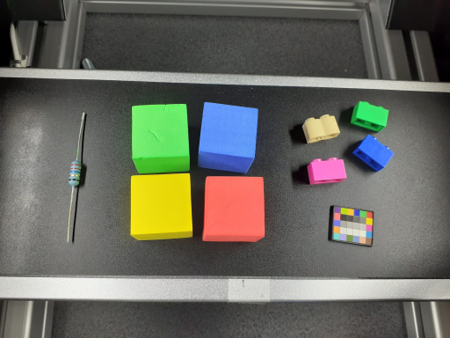
\includegraphics[width=0.5\textwidth]{../images/banc_vi_intro.png}
\end{center}

\vfill

\textit{Ce sujet est disponible au format électronique sur le site du LEnsE - https://lense.institutoptique.fr/ dans la rubrique Année / Première Année / Opto-Electronique S5 / TP / Bloc Vision Industrielle.}

\vspace{1.5cm}

\begin{minipage}{5cm}
\begin{center}

\includegraphics[width=3cm]{../images/logocc}\\
\small
  © 2025 by LEnsE-IOGS 
\end{center}
\end{minipage}

% Bottom of the page
%{\textbf{\large {Année universitaire} 2024-2025}}

\end{center}
\end{titlepage}

\newpage
\strut % empty page

\textit{L'image de la page de garde provient du projet DEPhI Vision Industrielle de 2026. Crédits : Joséphine BECHU, Justine GABRIEL et Paul CHENEAU (Promo 2027).}

\vfill


\newpage
\strut % empty page
%%%%%%%%%%%%%%%%%%%%%%%%%%%%%%%%%%%%%%%%%%%%%%%%
%%%%%%%%%%%%%    A A V

\section{Vision Industrielle}

La \textbf{vision industrielle} est une technologie qui permet à des machines d'\textbf{analyser automatiquement des scènes} pour \textbf{contrôler}, \textbf{guider} ou \textbf{inspecter} des objets sur des processus de production. Elle repose sur l'utilisation de \textbf{caméras}, d'\textbf{optique}, d'\textbf{éclairages} spécifiques (ou contraints), de \textbf{capteurs} et d'algorithmes de \textbf{traitement d'image}. 

\begin{center}
	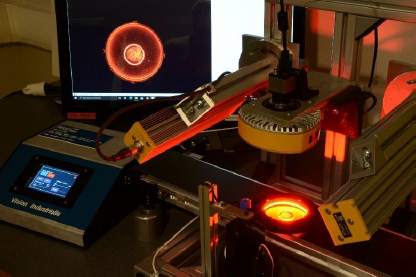
\includegraphics[width=0.5\textwidth]{../images/vi_intro_2.png}
\end{center}

Elle a pour but de \textbf{prendre des décisions automatiques} (ou aider l'être humain dans sa prise de décision) vis-à-vis d'un (ou plusieurs) objet(s) dans une scène spécifique : détecter des défauts ou des irrégularités, compter ou trier..., en rejetant ou validant automatiquement des produits, tout en assurant une constance de la qualité et de la répétabilité des opérations. 


\section{Ressources}


Ce bloc de travaux pratiques utilise un \textbf{banc de vision industrielle} avec une lampe de type Effi-Ring RGB, une caméra Basler et une interface développée en \textbf{Python} (\textit{PyQt6}) et qui utilise des fonctionnalités de la bibliothèque \textbf{OpenCV}.

Les documentations de la caméra et de l'éclairage sont disponibles aux adresses suivantes : 

\begin{itemize}
	\item Basler \textbf{a2A 1920 - 160ucBAS} : \href{https://docs.baslerweb.com/a2a1920-160ucbas#specifications}{https://docs.baslerweb.com/a2a1920-160ucbas\#specifications}
	\item \textbf{Effi-Ring} : \href{https://www.effilux.com/fr/produits/annulaire/effi-ring}{https://www.effilux.com/fr/produits/annulaire/effi-ring}
\end{itemize}

\bigskip

\noindent \rule{\linewidth}{1pt}

\bigskip

\textbf{\large Liste des ressources présentes dans ce document}
\begin{itemize}
	\item Camera BASLER a2A1920-uc/umBAS (Résumé)
	\item Source EFFI-Ring - Spectre et données / Version RGB
	\item Cubes de couleur - Réflectance
	\item Rappels sur les caméra CMOS
	\item Rappels sur le traitement d'images
\end{itemize}


\newpage
\pagestyle{empty}

\strut % empty page

\newpage
\pagestyle{empty}

\strut % empty page

\section*{Camera BASLER a2A1920-uc/umBAS}

\textit{La documentation complète se trouve sur le site du fabriquant - Basler}

\begin{center}
\begin{tabular}{|c|c|}
	\hline
	Marque & Basler\\
	Modèle & a2A1920-160ucBAS\\
	\hline
	Résolution & 1920 px x 1200 px\\
	Taille pixel & 3.45 x 3.45 $\operatorname{\mu{}m^2}$\\
	Profondeur & 12 bits\\
	\hline
	Efficacité quantique & 62.22 \%\\
	Gain (1/K) & 2.652 e-/DN\\
	Capacité de saturation & 10492 e-\\
	Capacité de saturation & 16862 p	\\
	\hline
\end{tabular}
\end{center}


\section*{Source EFFI-Ring - Spectre et données / Version RGB}

\textit{La documentation complète se trouve sur le site du fabriquant - Effilux}

\subsection*{Spectre} 

Obtenu à l'aide d'un spectromètre 

\begin{center}
	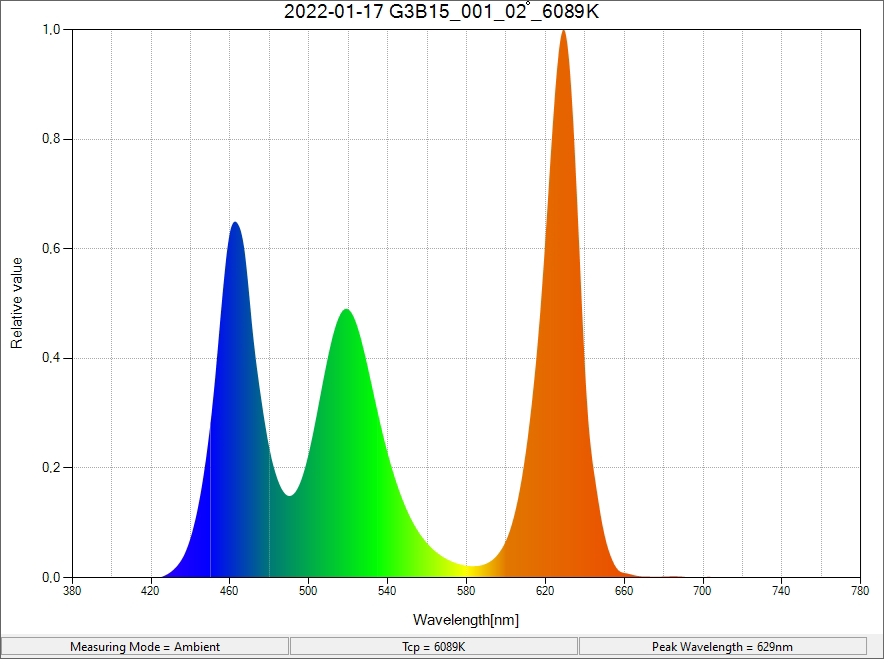
\includegraphics[width=0.7\textwidth]{../images/effi_ring_spectre.png}
\end{center}

\newpage
\subsection*{Taille du spot et éclairement en fonction de la distance de travail} 

Données provenant de la documentation technique.

\begin{center}
	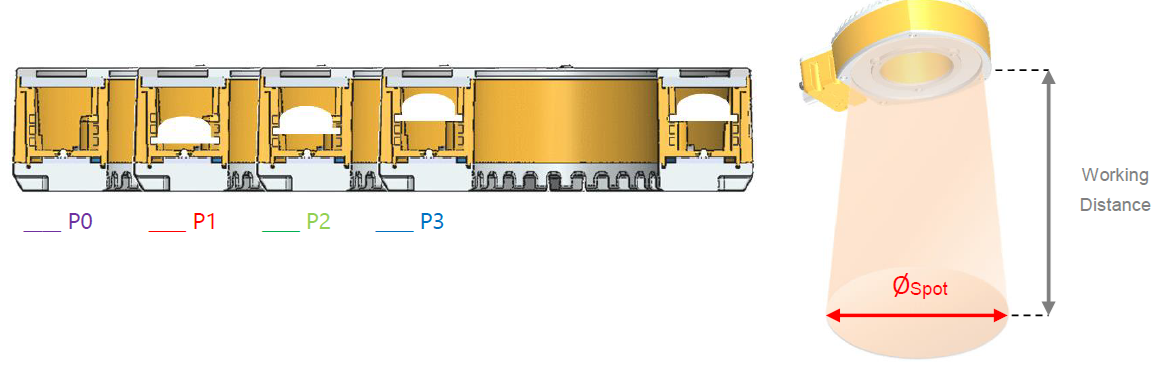
\includegraphics[width=0.65\textwidth]{../images/effi_ring_spot.png}
\end{center}

\begin{center}
	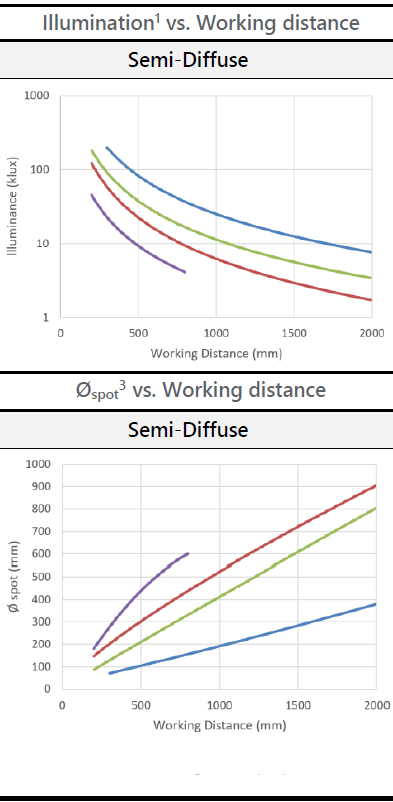
\includegraphics[width=0.48\textwidth]{../images/effi_ring_illu.png}
\end{center}


\section*{Cubes de couleur - Réflectance}

\begin{center}
	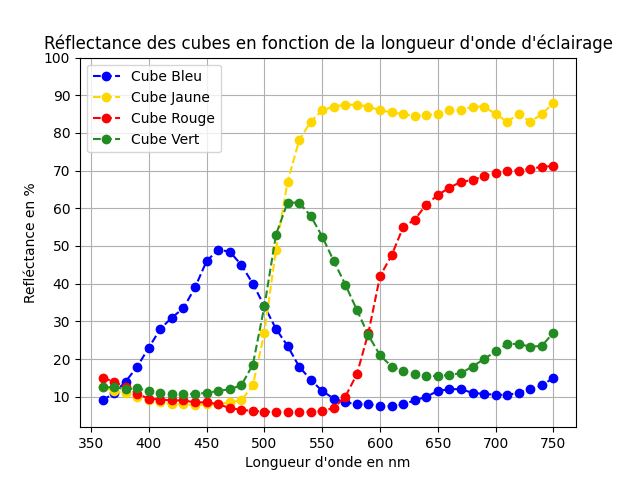
\includegraphics[width=0.7\textwidth]{../images/cubes_reflectance.png}
\end{center}

%


\newpage
\strut % empty page

%
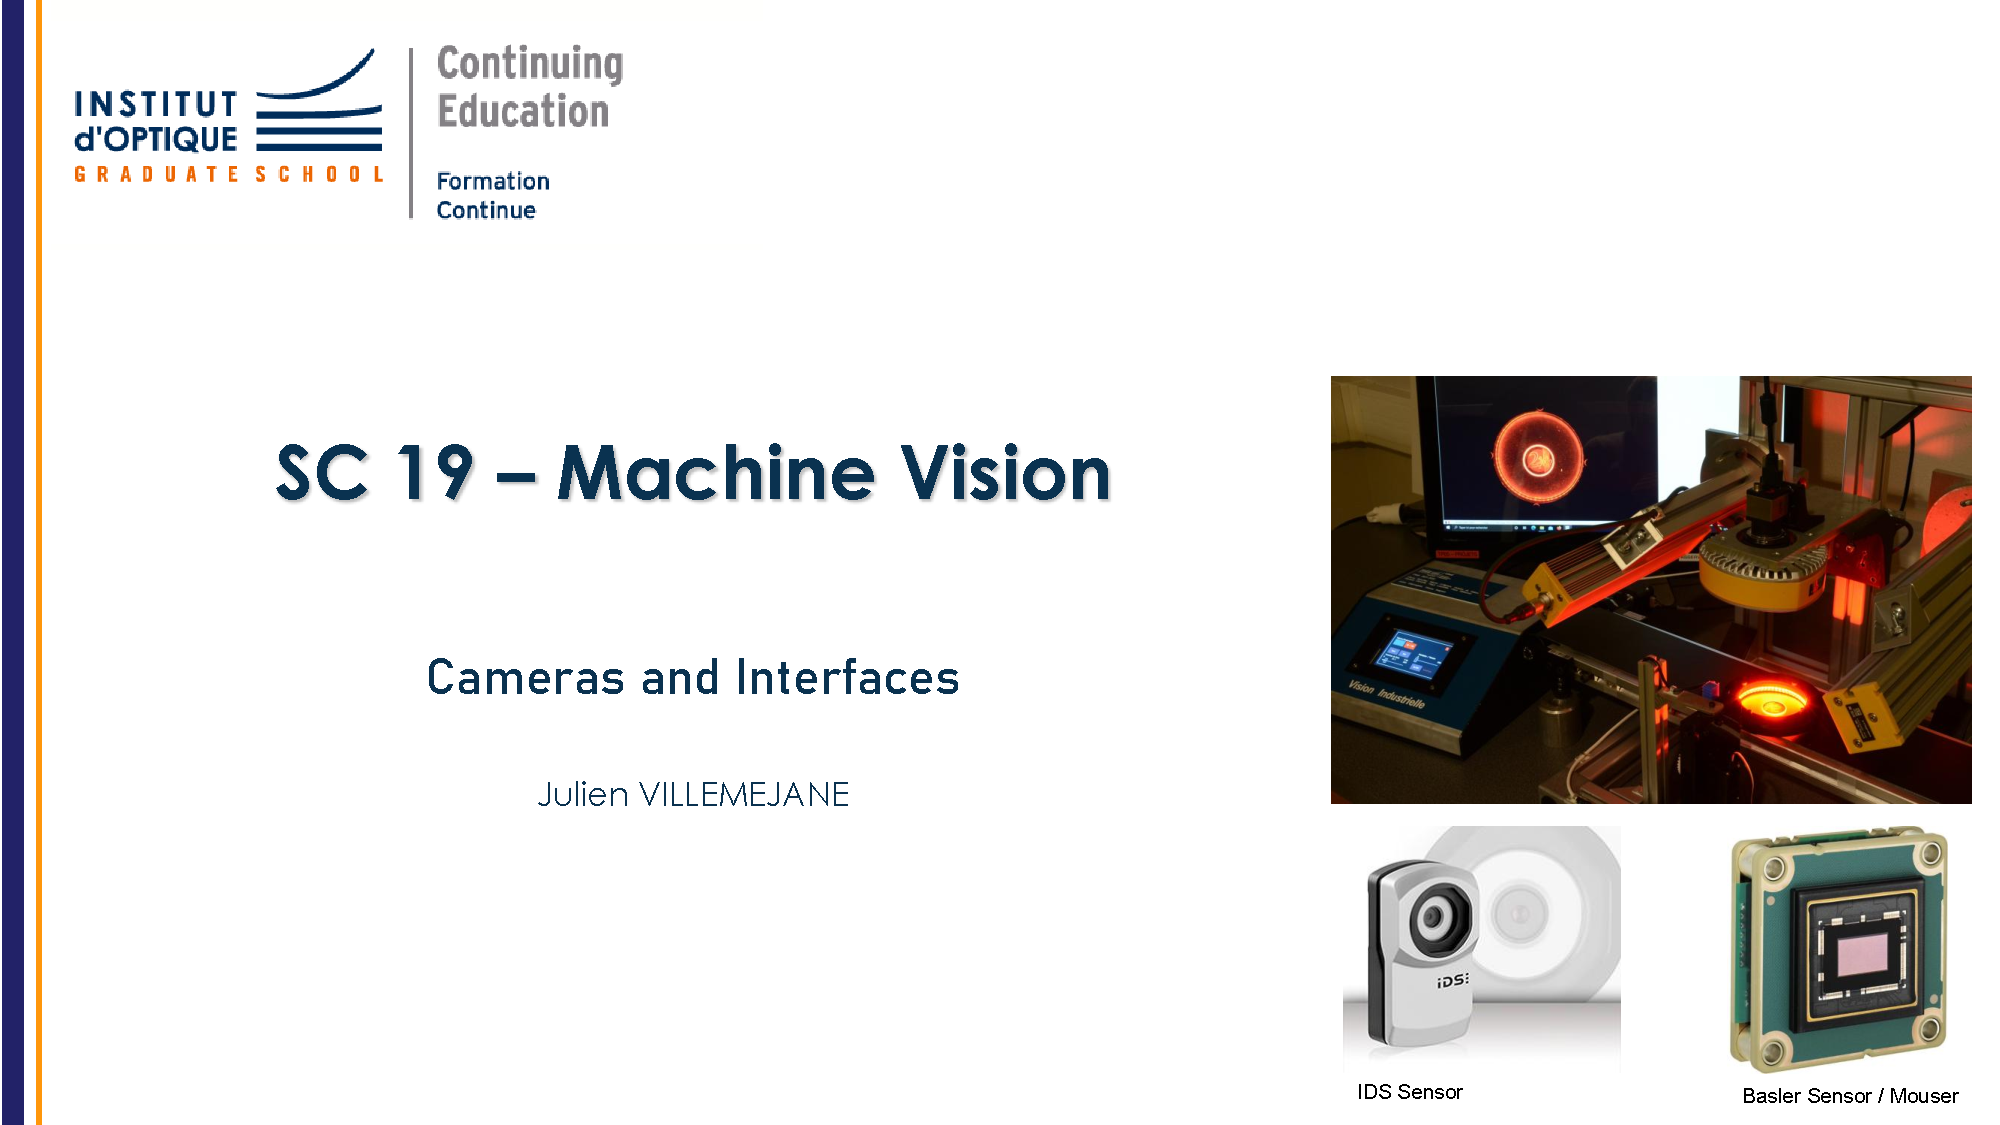
\includepdf[pages={1,3}, nup=1x2, pagecommand={\section{\texorpdfstring{\hspace{-1em}}{Camera CMOS}}}\label{doc:cam_cmos}]{../../docs/SC19_Camera_2025.pdf}
\includepdf[pages={6,8, 10-15, 18, 20, 26-28, 30, 32, 34-36}, nup=1x2]{../../docs/SC19_Camera_2025.pdf}



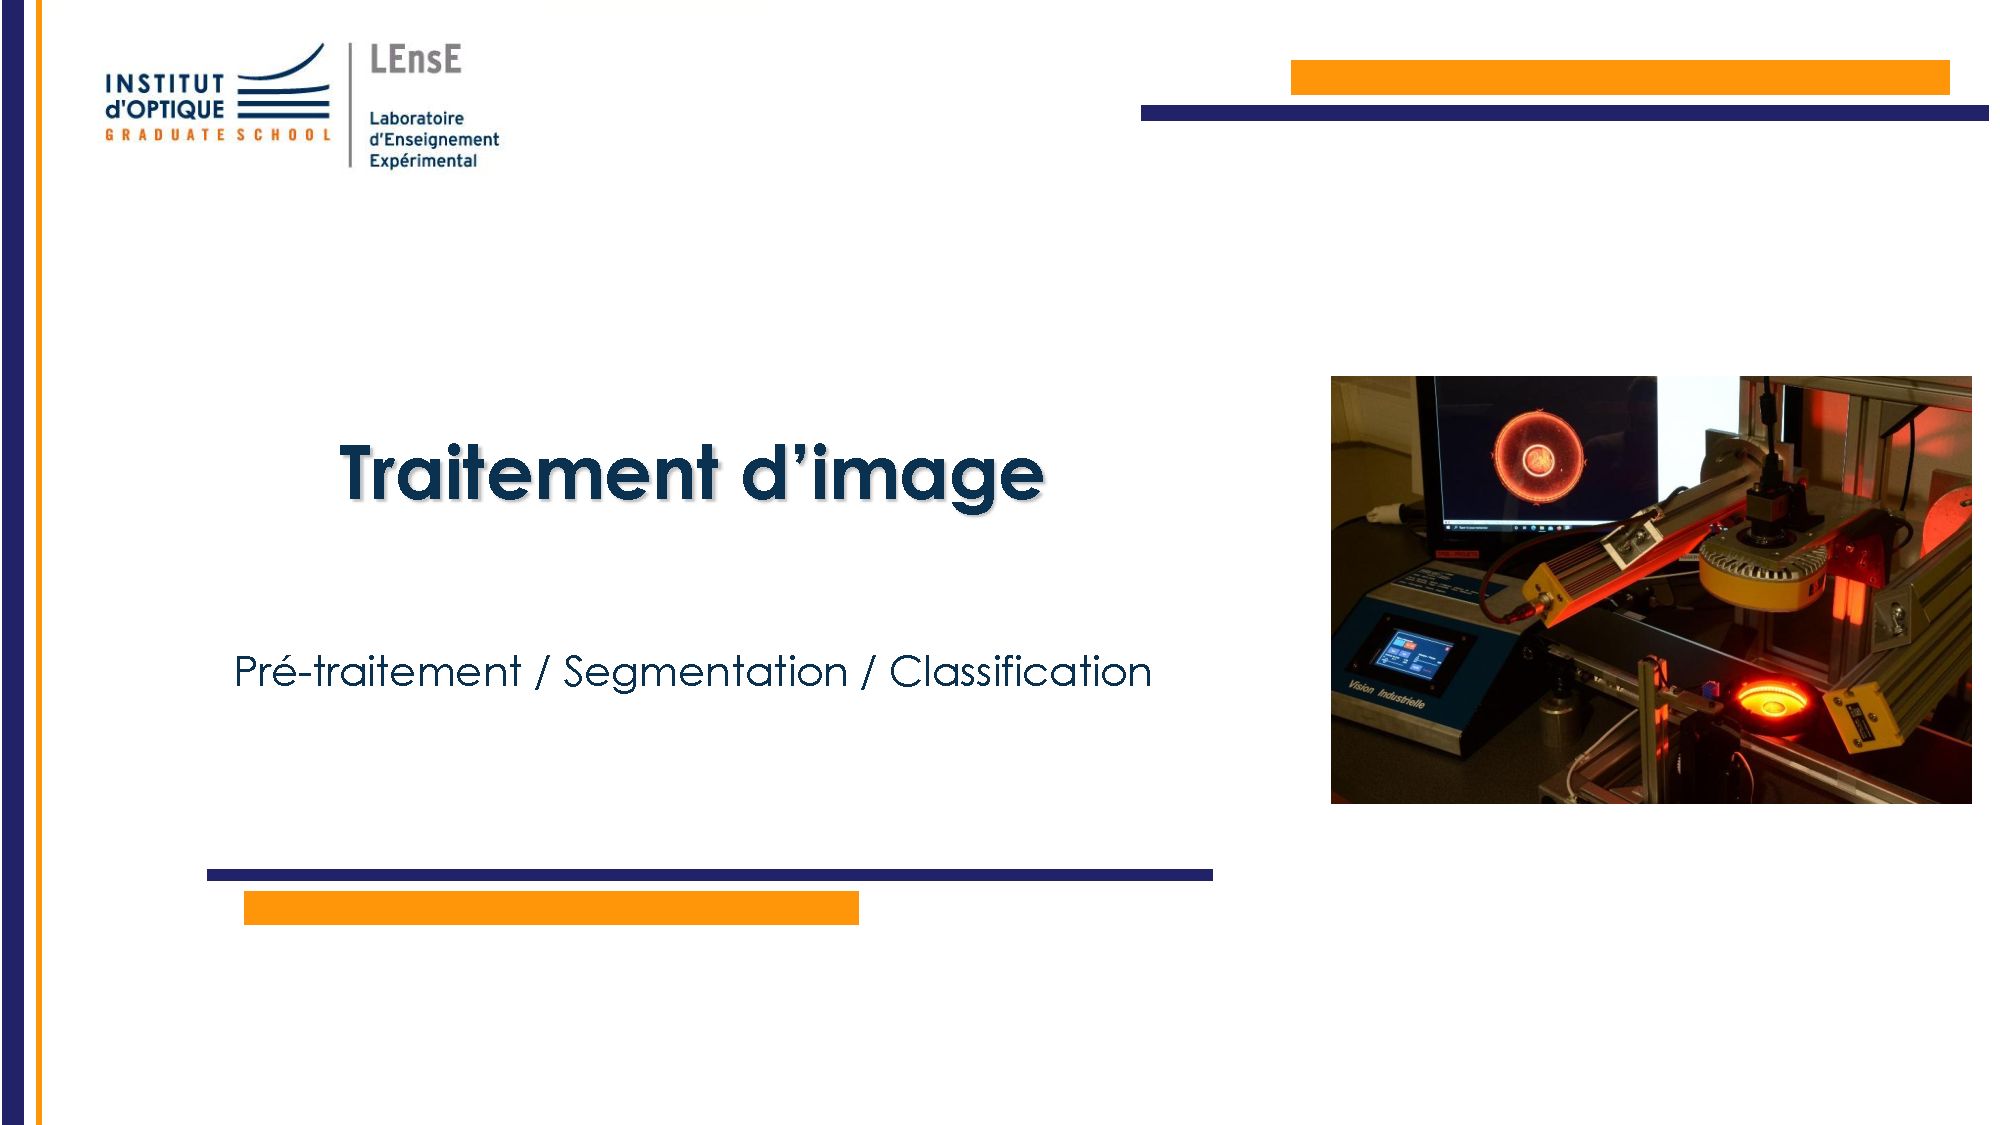
\includepdf[pages={1-2}, nup=1x2, pagecommand={\section{\texorpdfstring{\hspace{-1em}}{Image Processing}}}\label{doc:image_proc}]{../../docs/S6_IntNum_Processing_VI_2025.pdf}
\includepdf[pages={3, 5-6, 9, 7-8, 10-12, 15, 13-14, 16-18, 20-24}, nup=1x2]{../../docs/S6_IntNum_Processing_VI_2025.pdf}

\end{document}


